% !TeX Options = -shell-escape
\documentclass{panicsoftware-presentation}

\usepackage{tikz}
\usetikzlibrary{decorations.pathreplacing,patterns}

\title{Lifetime of the C++ object}
\author{Dawid Pilarski}
\date{}

\institute{dawid.pilarski@tomtom.com \\ dawid.pilarski@panicsoftware.com \\ \href{http://blog.panicsoftware.com}{blog.panicsoftware.com} }

\newenvironment{itemizeSeq}{\begin{itemize}[<+-|alert@+>]}{\end{itemize}}
\newenvironment{itemizeNColorSeq}{\begin{itemize}[<+->]}{\end{itemize}}

\begin{document}

\begin{frame}
	\maketitle
\end{frame}

\begin{frame}{Agenda}
	\tableofcontents
\end{frame}

\begin{frame}{Who am I?}
			\centering \alert{Dawid Pilarski}
			\vskip 1em
	\begin{columns}[onlytextwidth]
		\begin{column}{0.7\textwidth}
			\begin{itemize}
				\item Senior Software Developer in TomTom
				\item Member of the ISO/JTC1/SC22/WG21
				\item Member of the PKN KT {\tiny(programming languages)}
				\item C++ blog writer
			\end{itemize}
		\end{column}
		\begin{column}{0.29\textwidth}
				
\includegraphics[width=\linewidth]{Dawid_Pilarski.jpg}				
		\end{column}	
	\end{columns}
\end{frame}

\begin{frame}{Questions.}
	
	\vfill
	\centerline{Questions...}
	\vfill

\end{frame}

\begin{frame}{Question...}

\centerline{Do you think, that understanding objects and their lifetimes is \alert{basics}?}

\end{frame}

\begin{frame}{What we talk about are basics.}

	\centering
	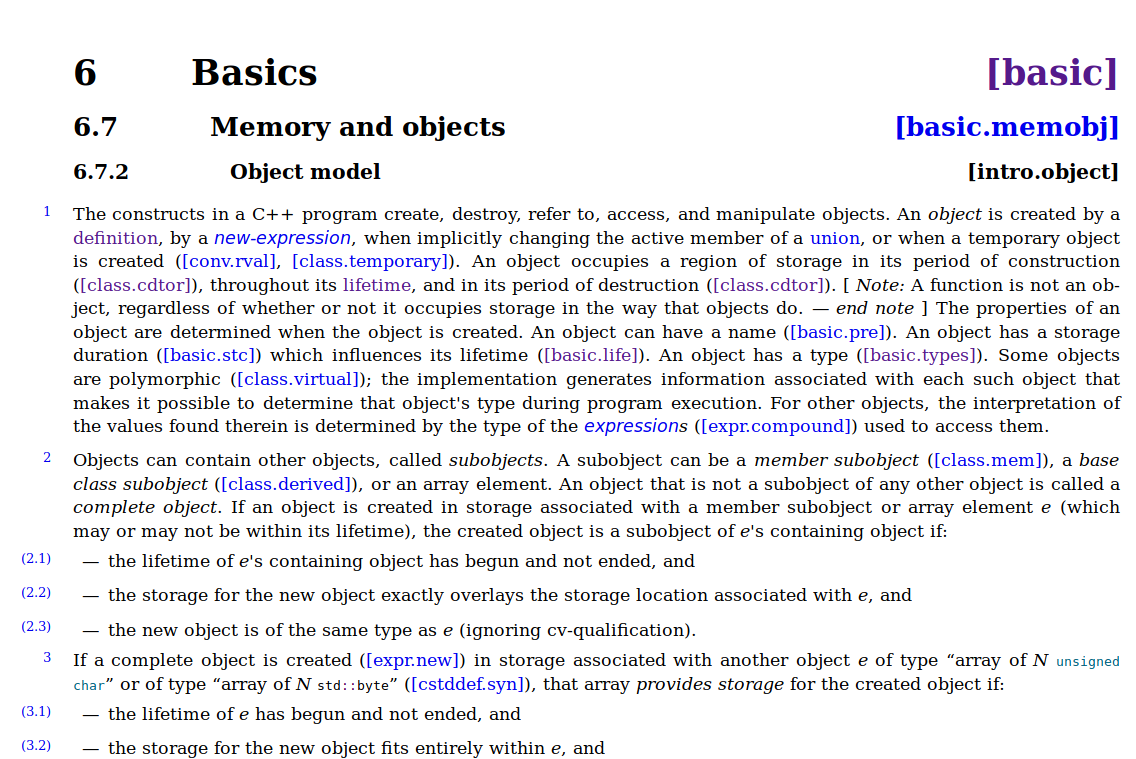
\includegraphics[width=1.0\linewidth]{graphics/objects_basics.png}

\end{frame}


\section{Theory}

\begin{frame}{Title decomposition}

\centerline{What's the \only{lifetime}<1>\only{\alert{lifetime}}<2-> of your \only{object}<1-2>\only{\alert{object}}<3>?}
\pause
\begin{itemizeSeq}
	\item What is a lifetime?
	\item What is an object?
\end{itemizeSeq}

\end{frame}

\section*{Objects}

\begin{frame}{The object}

Objects are entities, that can be:
\begin{itemize}
	\item created
	\item destroyed
	\item refered to
	\item accessed
	\item manipulated
\end{itemize}

\end{frame}

\begin{frame}{The Object}

\begin{columns}
	\begin{column}{0.58\linewidth}
	
	Is created:
	\begin{itemizeSeq}
		\item by the definition
		\item by the new expression
		\item when changing active\\ member of a union
		\item by creation of the temporary
	\end{itemizeSeq}
	\end{column}

	\begin{column}{0.48\linewidth}
	
	\only{\centering\inputminted{\myCpp}{examples/object-definition.cpp}}<1>
	\only{\centering\inputminted{\myCpp}{examples/new-expression.cpp}}<2>
	\only{\centering\inputminted{\myCpp}{examples/union-active-member-change.cpp}}<3>
	\only{\centering\inputminted{\myCpp}{examples/temporary-creation.cpp}}<4>
	\end{column}

\end{columns}

\end{frame}


\newcounter{tmpCounter}
\begin{frame}{The object}

\begin{columns}
\begin{column}{0.3\linewidth}

Has:
\begin{itemizeSeq}
	\item optional name
	\item lifetime
	\item storage and it's duration
	\begin{itemizeSeq}
		\item static
		\item thread
		\item automatic
		\item dynamic
	\end{itemizeSeq}
	\item type
	\item value
\end{itemizeSeq}

\end{column}

\begin{column}{0.5\linewidth}
\only{\alert{program duration}}<4>
\only{\alert{thread duration}}<5>
\only{\alert{enclosing scope duration}}<6>
\only{\alert{controlled by user}}<7>
\end{column}

\end{columns}
\end{frame}

\begin{frame}{The reference}

\centerline{Is not an object {\scriptsize(although reference has lifetime)}}

\centerline{\footnotesize functions are not objects as well}

\end{frame}

\begin{frame}[fragile]{The variable}

\centerline{Is created by a \alert{declaration} of an \alert{object} or the \alert{reference}.}
\pause
\vfill

\begin{columns}[t]

\begin{column}{0.3\linewidth}
\begin{minted}{\myCpp}
int x;
\end{minted}
\vskip 1cm
Is a variable.

\end{column}
\pause

\begin{column}{0.3\linewidth}
\begin{minted}{\myCpp}
int& x = ...
\end{minted}
\vskip 1cm
Is variable.

\end{column}
\pause

\begin{column}{0.3\linewidth}
\begin{minted}{\myCpp}
struct X{int y;}z;
\end{minted}
\vskip 1cm
Neither \texttt{X} nor \texttt{y} are variables.\\
\texttt{z} is a variable.
\end{column}

\end{columns}

\end{frame}

\begin{frame}{Summary: variable, reference, object}
\centering
\begin{figure}
\resizebox{0.9\linewidth}{!}{
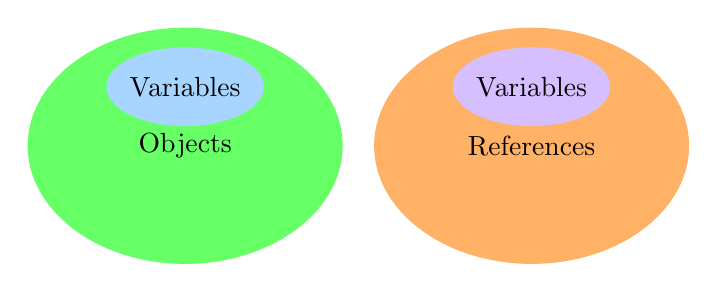
\begin{tikzpicture}
\begin{scope}[blend group=soft light]

\fill[blue!30!white] (-2.2,-0.25) circle[x radius=1cm, y radius=0.5cm];
\fill[blue!30!white] (2.2,-0.25) circle[x radius=1cm, y radius=0.5cm];
\fill[green!60!white] (-2.2,-1) circle[x radius=2cm, y radius=1.5cm];
\fill[orange!60!white] (2.2,-1) circle[x radius=2cm, y radius=1.5cm];

\end{scope}

\node at(-2.2,-0.25){Variables};
\node at(2.2,-0.25){Variables};
\node at(2.2,-1){References};
\node at(-2.2,-1){Objects};

\end{tikzpicture}}

\end{figure}

\end{frame}


\begin{frame}{Definitions}
	If you want to get precise definitions, you need to look at standard draft. In case of \href{http://cppreference.com}{\alert{cppreference}}:

	\begin{itemizeSeq}
		\item The object has been recently updated.
		\item The variable definition is unmaintained and unsupported.
		\item Same about references...
		\item Wikipedia is wrong regarding C++ language.
	\end{itemizeSeq}
\end{frame}

\section*{Lifetime}

\begin{frame}{What is a lifetime?}

\centerline{Lifetime is a \alert{runtime} property of an object.}

\vfill
\centering

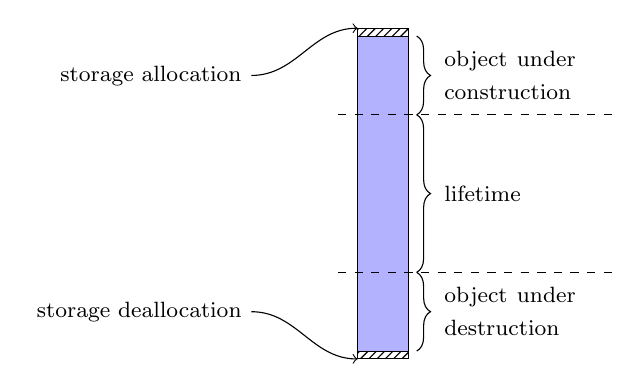
\begin{tikzpicture}

\draw[fill=blue!30!white] (-.75, -2) rectangle (-0.1, 2);
\draw[pattern=north east lines] (-.75, 2) rectangle (-0.1, 2.1);
\draw[pattern=north east lines] (-.75, -2) rectangle (-0.1, -2.1);

\draw[<-] (-0.75, 2.1) to[out=-180, in=0] (-2.1, 1.5) node[left]{\footnotesize storage allocation}; \pause
\draw [decorate, decoration={brace, amplitude=5pt}] (0, 2) -- (0, 1) node[xshift=1.35cm ,midway, text width=2cm]{\footnotesize object under construction};
\draw[dashed] (-1, 1) -- (2.5, 1); \pause
\draw [decorate, decoration={brace, amplitude=5pt}] (0, 1) -- (0,-1) node[xshift=1.35cm ,midway, text width=2cm]{\footnotesize lifetime};
\draw[dashed] (-1, -1) -- (2.5, -1);\pause
\draw [decorate, decoration={brace, amplitude=5pt}] (0, -1) -- (0, -2) node[xshift=1.35cm ,midway, text width=2cm]{\footnotesize object under destruction};
\pause
\draw[<-] (-0.75, -2.1) to[out=-180, in=0] (-2.1, -1.5) node[left]{\footnotesize storage deallocation};

\end{tikzpicture}
\vfill
\centerline{During the lifetime of an object you can use it without additional restrictions.}

\end{frame}

\begin{frame}{When does the lifetime start?}

\centerline{The lifetime of an object \alert{starts}, when:}

\begin{itemizeSeq}

\item storage with the proper alignment and size for type T is obtained
\item its initialization (if any)* is complete
\item if the object is a union member or subobject thereof, its lifetime only begins if that union member is the initialized member

\end{itemizeSeq}

\uncover<2>{\alert{*In case of default construction of trivial type, there is no initialization performed}}

\end{frame}

\begin{frame}{When does the lifetime end?}

\centerline{The lifetime of an object \alert{ends}:}

\begin{description}[<+-|alert@+>]

\item[class types] when it's destructor is called,
\item[non-class types] when we expect it to end its lifetime, 
\begin{itemize}
	\item when object exits the scope,
	\item delete expression,
	\item when temporary ends its lifetime etc.
\end{itemize}
\item[any type] when storage occupied by an object is reused or released.
\end{description}

\end{frame}

\begin{frame}{Limitations on objects - Storage allocated cdtor not yet called}

During this phase you must treat every pointer/reference to such object as if it was raw storage.

During construction you cannot:
\begin{itemizeSeq}
	\item pass pointer as \texttt{delete} argument,
	\item access any non-static members (unless type has trivial ctor),
	\item \texttt{static\_cast} to types other than:
	\begin{itemize}
		\item \texttt{void*}
		\item \texttt{char*}
		\item \texttt{unsigned char*}
		\item \texttt{std::byte*}
	\end{itemize} 
	\item \texttt{dynamic\_cast} it.
\end{itemizeSeq}

\end{frame}

\begin{frame}{Limitations on objects - object under (con|de)struction}
You \alert{can access non-static members of a class}, but only via \alert{this} pointer.

Example from C++ standard draft:

\only{\inputminted[highlightlines={1-4}]{\myCpp}{examples/access-via-this-under-construction.cpp}}<2>
\only{\inputminted[highlightlines={3}]{\myCpp}{examples/access-via-this-under-construction.cpp}}<3>
\only{\inputminted[highlightlines={7-10}]{\myCpp}{examples/access-via-this-under-construction.cpp}}<4>
\only{\inputminted[highlightlines={6}]{\myCpp}{examples/access-via-this-under-construction.cpp}}<5>
\only{\inputminted[highlightlines={8,9}]{\myCpp}{examples/access-via-this-under-construction.cpp}}<6>

\end{frame}

\begin{frame}{Limitations on objects - object under (con|de)struction}
\only{\inputminted[highlightlines={1-4}]{\myCpp}{examples/typeid2.cpp}}<1>
\only{\inputminted[highlightlines={5}]{\myCpp}{examples/typeid2.cpp}}<2>
\only{\inputminted[highlightlines={7-11}]{\myCpp}{examples/typeid2.cpp}}<3>
\only{\inputminted[highlightlines={8}]{\myCpp}{examples/typeid2.cpp}}<4>
\only{\inputminted[highlightlines={9}]{\myCpp}{examples/typeid2.cpp}}<5>

\uncover<4-5>{
\begin{block}{Output:}
\only{\alert{4Base}}<4>
\only{\alert{0}}<5>
\end{block}
}
\end{frame}

\begin{frame}[fragile]{Limitations on objects - object under (con|de)struction}

\begin{columns}[t]
\begin{column}{0.48\linewidth}
\inputminted[fontsize=\small]{\myCpp}{examples/runnable.cpp}
\vfill
\end{column}
\begin{column}{0.48\linewidth}
\begin{minted}[fontsize=\small]{\myCpp}
runnable* d = new Derived;
thread th1([d]{d->execute()});
thread th2([d]{delete d;});
\end{minted}
\end{column}

\end{columns}

\end{frame}

\section{Object model intuition}

\begin{frame}{The usual mindset towards object}

\begin{columns}

\begin{column}{0.3\linewidth}
\begin{itemizeSeq}
\item We have got a memory
\item Objects are the way to represent value in that memory
\end{itemizeSeq}
\end{column}
\begin{column}{0.56\linewidth}

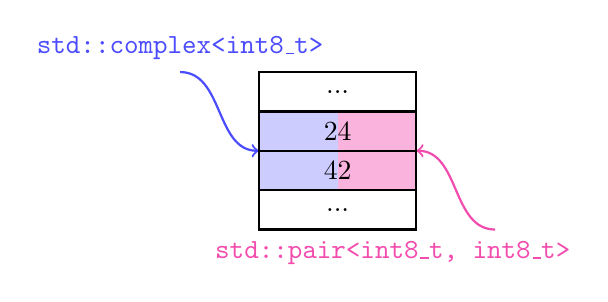
\begin{tikzpicture}

\onslide<3-4>{
\fill[blue!20] (-2,0.5) rectangle (-1,1.5);
\draw[thick, blue!70, ->] (-3, 2) node[yshift=3mm]{\texttt{std::complex<int8\_t>}} to[out=0, in=180] (-2, 1);
}

\onslide<4>{
\fill[magenta!30] (-1,0.5) rectangle (0,1.5);
\draw[thick, magenta!70, ->] (1, 0) node[yshift=-3mm, xshift=-1.3cm]{\texttt{std::pair<int8\_t, int8\_t>}} to[out=180, in=0] (0, 1);
}

\draw[thick] (-2,0) rectangle node{...} (0,0.5);
\draw[thick] (-2,0.5) rectangle node{42} (0,1);
\draw[thick] (-2,1) rectangle node{24} (0,1.5);
\draw[thick] (-2,1.5) rectangle node{...} (0,2);

\end{tikzpicture}

\end{column}

\end{columns}


\end{frame}

\begin{frame}{Examples of invalid C++ - union type punning}

\only{\inputminted[highlightlines={1-6}]{\myCpp}{examples/invalid_union_use.cpp}}<1>
\only{\inputminted[highlightlines={8-11}]{\myCpp}{examples/invalid_union_use.cpp}}<2>
\only{\inputminted[highlightlines={13-14}]{\myCpp}{examples/invalid_union_use.cpp}}<3>

\end{frame}

\begin{frame}{Examples of invalid C++ - reinterpret\_cast}

\only{\inputminted[highlightlines={1-3}]{\myCpp}{examples/invalid-reinterpret-cast.cpp}}<1>
\only{\inputminted[highlightlines={5,11}]{\myCpp}{examples/invalid-reinterpret-cast.cpp}}<2>
\only{\inputminted[highlightlines={6}]{\myCpp}{examples/invalid-reinterpret-cast.cpp}}<3>
\only{\inputminted[highlightlines={7}]{\myCpp}{examples/invalid-reinterpret-cast.cpp}}<4>
\only{\inputminted[highlightlines={9,10}]{\myCpp}{examples/invalid-reinterpret-cast.cpp}}<5>

\end{frame}

\begin{frame}{reinterpret\_cast attempt 2}

\only{\inputminted[highlightlines={9}]{\myCpp}{examples/invalid_reinterpret_cast-2.cpp}}<1>

\end{frame}

\section*{But... why?}

\begin{frame}{Why all the attempts are wrong?}

\centerline{Compiler \alert{doesn't} think in terms of \alert{objects and memory}}
\vskip 1cm
\pause 

\centerline{Compiler thinks in terms of \alert{objects and their types}.}

\end{frame}

\begin{frame}{Test with two different class types}

\only{\inputminted[highlightlines={1-3,5-7}]{\myCpp}{examples/TBAA-simple-example.cpp}}<1>
\only{\inputminted[highlightlines={9,14}]{\myCpp}{examples/TBAA-simple-example.cpp}}<2>
\only{\inputminted[highlightlines={10,11,13}]{\myCpp}{examples/TBAA-simple-example.cpp}}<3->

\vfill
\only{\centerline{Q: \alert{What is the return value?}}}<4>

\end{frame}

\begin{frame}{Test with two same structures}

\only{\inputminted[highlightlines={1-3}]{\myCpp}{examples/Non-TBAA-simple-example.cpp}}<1>
\only{\inputminted[highlightlines={5}]{\myCpp}{examples/Non-TBAA-simple-example.cpp}}<2>
\only{\inputminted[highlightlines={6,7,9}]{\myCpp}{examples/Non-TBAA-simple-example.cpp}}<3->
\vfill
\only{\centerline{Q: \alert{What is the return value now?}}}<4>

\end{frame}

\begin{frame}{Assumptions, that compiler does}

\begin{columns}[t]

\begin{column}{0.58\linewidth}


\centerline{Code:}

\vfill

\inputminted[firstline=9, highlightlines={9}]{\myCpp}{examples/TBAA-simple-example.cpp}

\end{column}


\begin{column}{0.28\linewidth}

\centerline{Assembly:}

\vfill

\centering\inputminted[highlightlines={6}]{gas}{examples/TBAA-simple-example.asm}

\end{column}

\end{columns}

\end{frame}

\begin{frame}{Assumptions, that compiler does}

\begin{columns}[t]

\begin{column}{0.58\linewidth}


\centerline{Code:}

\vfill

\inputminted[firstline=5, highlightlines=5]{\myCpp}{examples/Non-TBAA-simple-example.cpp}

\end{column}


\begin{column}{0.28\linewidth}

\centerline{Assembly:}

\vfill

\centering\inputminted[highlightlines={6,7}]{gas}{examples/Non-TBAA-simple-asembly.asm}

\end{column}

\end{columns}

\end{frame}

\begin{frame}{Conclusion}

We cannot allow 2 objects of different types (not subobjects) live:

\begin{itemize}
	\item in the same space.
	\item at the same time.
\end{itemize}

\end{frame}

\begin{frame}{Explanations: type punning in union}

\begin{columns}

\begin{column}{0.48\linewidth}
\inputminted[highlightlines={14}]{\myCpp}{examples/invalid_union_use.cpp}
\end{column}
\begin{column}{0.48\linewidth}

\centerline{\alert{errors:}}

\begin{itemizeSeq}
\item Accessing inactive member of union,
\item Reading not existing object.
\end{itemizeSeq}

\end{column}

\end{columns}


\end{frame}

\begin{frame}{How to do it right?}

\only{\inputminted[highlightlines={2-4}]{\myCpp}{examples/invalid_union_use_right.cpp}}<1>
\only{\inputminted[highlightlines={6,10}]{\myCpp}{examples/invalid_union_use_right.cpp}}<2>
\only{\inputminted[highlightlines={7-9}]{\myCpp}{examples/invalid_union_use_right.cpp}}<3->

\end{frame}

\begin{frame}{Explanations: reading from a stream}

\begin{columns}[t]

\begin{column}{0.48\linewidth}
\inputminted{\myCpp}{examples/invalid-reinterpret-cast.cpp}
\end{column}

\begin{column}{0.48\linewidth}
\centerline{\alert{errors:}}

\begin{itemizeSeq}
\item reading object of type T, that was not created
\end{itemizeSeq}
\end{column}

\end{columns}

\end{frame}

\begin{frame}{How to do it right?}

\only{\inputminted[highlightlines={1-3}]{\myCpp}{examples/invalid-reinterpret-cast-right.cpp}}<1>
\only{\inputminted[highlightlines={9,10}]{\myCpp}{examples/invalid-reinterpret-cast-right.cpp}}<2>

\begin{tikzpicture}[remember picture, overlay]
\draw[color=magenta, thick, ->] (2,6.25) to[out=0, in=180] (4,5.25) node[right](){trivially copyable};
\end{tikzpicture}

\end{frame}

\begin{frame}{Or with C++20}
\inputminted[highlightlines={9}]{\myCpp}{examples/invalid-reinterpret-cast-right-modern.cpp}
\end{frame}

\begin{frame}{Explanations: reading from a stream - placement new}

\begin{columns}

\begin{column}{0.48\linewidth}

\inputminted{\myCpp}{examples/invalid-reinterpret-cast-2-short.cpp}
\end{column}

\begin{column}{0.48\linewidth}

\begin{itemizeSeq}
\item placement new reuses the storage (ends lifetime of buff),
\item value is a runtime property of an object (doesn't exist outside of it's lifetime)
\item T is created uninitialized
\item reading T is reading indeterminate value, which is UB
\end{itemizeSeq}
\end{column}
\end{columns}
\end{frame}

\section*{std::launder}

\begin{frame}{Tricky placement new}

\begin{columns}

\begin{column}{0.48\linewidth}
\inputminted{\myCpp}{examples/placement-new-issue.cpp}
\end{column}

\begin{column}{0.48\linewidth}
\begin{itemizeSeq}
\item sometimes you know, there is an object of given type under given address.
\item but you cannot just \texttt{reinterpret\_cast} the pointer to get to the object.
\end{itemizeSeq}
\end{column}
\end{columns}
\end{frame}

\begin{frame}{What's the solution to the problem?}

\begin{description}[<+-|alert@+>]
\item[Until C++14] No solution. Go on with UB.
\item[Since C++17] \texttt{std::launder}.
\end{description}

\end{frame}

\begin{frame}[fragile]{What is std::launder?}
\centerline{Reading \alert{cppreference}:}

\begin{minted}{\myCpp}
template <class T>
constexpr T* launder(T* p) noexcept;
\end{minted}

\pause

\only{Obtains a pointer to the object located at the address represented by p.}<2>
\only{Obtains a \alert{pointer to the object} located at the address represented by p.}<3> 
\end{frame}

\begin{frame}{Usage of std::launder}

\only{\inputminted[highlightlines={5-6}]{\myCpp}{examples/placement-new-launder.cpp}}<1>
\only{\inputminted[highlightlines={7}]{\myCpp}{examples/placement-new-launder.cpp}}<2>
\only{\inputminted[highlightlines={8}]{\myCpp}{examples/placement-new-launder.cpp}}<3->

\uncover<4>{
\begin{tikzpicture}[remember picture, overlay]
\draw[color=magenta, thick, <-] (1,0.7) to[out=-90, in=-180] node[xshift=1.1cm, yshift=-0.1cm]{valid} (2,0);
\end{tikzpicture}	
}

\end{frame}

\begin{frame}{Other use-cases of the std::launder}

\only{\inputminted[highlightlines={1-3}]{\myCpp}{examples/non-assignable-launder.cpp}}<1>
\only{\inputminted[highlightlines={5,6}]{\myCpp}{examples/non-assignable-launder.cpp}}<2>
\only{\inputminted[highlightlines={8,9}]{\myCpp}{examples/non-assignable-launder.cpp}}<3>
\only{\inputminted[highlightlines={11,12}]{\myCpp}{examples/non-assignable-launder.cpp}}<4>

\begin{tikzpicture}[remember picture, overlay]
\draw[color=magenta, thick, <-] (2,6.25) to[out=0, in=180] node[xshift=1.75cm, yshift=-0.4cm]{not assignable} (3,5.5);

\only{
\draw[color=violet, thick, <-] (2.1,0.9) to[out=0, in=180] (3.1,1.15);
\draw[color=violet, thick, <-] (2.1,1.4) to[out=0, in=180] node[xshift=2cm, yshift=-0.1cm]{Are those correct?} (3.1,1.15);	
}<4>

\end{tikzpicture}

\end{frame}

\begin{frame}{Rules for placement new for such cases}

\centerline{You can do placement new on old object with same type and keep using old object.}
\pause
\centerline{With some exceptions (until C++20). For example:}

\begin{itemizeSeq}
\item We cannot use original object when it has:
\begin{itemizeSeq}
\item references
\item const members
\end{itemizeSeq}
\end{itemizeSeq}

\end{frame}

\begin{frame}{Example: const member or reference}

\only{\inputminted[highlightlines={1-4}]{\myCpp}{examples/non-assignable-launder-bad.cpp}}<1>
\only{\inputminted[highlightlines={11}]{\myCpp}{examples/non-assignable-launder-bad.cpp}}<2>
\only{\inputminted[highlightlines={12}]{\myCpp}{examples/non-assignable-launder-bad.cpp}}<3>
\only{\inputminted[highlightlines={13}]{\myCpp}{examples/non-assignable-launder-bad.cpp}}<4>

\end{frame}

\begin{frame}{Example: standard layout types}

\only{\inputminted[highlightlines={1-4}]{\myCpp}{examples/non-assignable-launder-good.cpp}}<1>
\only{\inputminted[highlightlines={11-13}]{\myCpp}{examples/non-assignable-launder-good.cpp}}<2>

\end{frame}

\section*{Implicit object creation}

\begin{frame}{Implicit object creation}
Until C++20 there is one case of implicit object creation:
\vskip 2em
\centerline{\alert{for defaulted, trivial assignment operators of union members.}}

\pause 

\vfill

What does that mean?

\end{frame}

\begin{frame}{Implicit object creation for unions}

\only{\inputminted[highlightlines={1-4}]{\myCpp}{examples/implicit-obj-creation-unions.cpp}}<1>
\only{\inputminted[highlightlines={6-9}]{\myCpp}{examples/implicit-obj-creation-unions.cpp}}<2>
\only{\inputminted[highlightlines={11-13}]{\myCpp}{examples/implicit-obj-creation-unions.cpp}}<3>


\only{
\begin{tikzpicture}[remember picture, overlay]
\draw[color=magenta, thick, <-] (3.2,2)   to[out=0, in=180] (4.5,1.4);
\draw[color=magenta, thick, <-] (3.2,1.4) to[out=0, in=180] (4.5,1.4);
\draw[color=magenta, thick, <-] (3.2,0.8) to[out=0, in=180] node[xshift=1.25cm, yshift=0.3cm]{correct} (4.5,1.4);
\end{tikzpicture}
}<3>
\end{frame}

\begin{frame}{Implicit object creation for unions}

\inputminted[highlightlines={4,13}]{\myCpp}{examples/implicit-obj-creation-unions-nondefault.cpp}

\end{frame}

\begin{frame}{Implicit object creation for C++20}

\begin{columns}

\begin{column}{0.45\linewidth}


Implicit object creation in the C++20 will be extended for:

\begin{itemizeSeq}

\item malloc-like functions
\item operator new
\item std::allocator<T>::allocate
\item memcpy, memmove
\item creation of arrays of:
\begin{itemize}[<5->]
	\item char
	\item unsigned char
	\item std::byte
\end{itemize}

\end{itemizeSeq}

\end{column}

\begin{column}{0.55\linewidth}

\only{\inputminted{\myCpp}{examples/implicit-obj-creation-malloc.cpp}}<1>
\only{\inputminted{\myCpp}{examples/implicit-obj-creation-new.cpp}}<2>
\only{\inputminted{\myCpp}{examples/implicit-obj-creation-alloc.cpp}}<3>
\only{\inputminted{\myCpp}{examples/implicit-obj-creation-memcpy.cpp}}<4>
\only{\inputminted{\myCpp}{examples/implicit-obj-creation-array.cpp}}<5>

\end{column}

\end{columns}


\end{frame}

\section{Beyond the object lifetime.}

\begin{frame}{Lifetime}

\begin{columns}
\begin{column}{0.58\linewidth}
\begin{tikzpicture}

\draw[fill=blue!30!white] (-.75, -2) rectangle (-0.1, 2);

\draw[dashed] (-1, 1) -- (2.5, 1);
\draw[dashed] (-1, -1) -- (2.5, -1);

\only{\draw [decorate, decoration={brace, amplitude=5pt}] (0, 2) -- (0, 1) node[xshift=1.35cm ,midway, text width=2cm]{\footnotesize \alert{object under construction}}}<1>;
\only{\draw [decorate, decoration={brace, amplitude=5pt}] (0, 2) -- (0, 1) node[xshift=1.35cm ,midway, text width=2cm]{\footnotesize object under construction}}<2->;

\only{\draw [decorate, decoration={brace, amplitude=5pt}] (0, 1) -- (0,-1) node[xshift=1.35cm ,midway, text width=2cm]{\footnotesize \alert{lifetime}}}<2>;
\only{\draw [decorate, decoration={brace, amplitude=5pt}] (0, 1) -- (0,-1) node[xshift=1.35cm ,midway, text width=2cm]{\footnotesize lifetime}}<3->;
\only{\draw [decorate, decoration={brace, amplitude=5pt}] (0, -1) -- (0, -2) node[xshift=1.35cm ,midway, text width=2cm]{\footnotesize \alert{object under destruction}}}<3>;

\end{tikzpicture}
\end{column}
\begin{column}{0.38\linewidth}

\only{Not for \alert{\texttt{trivially\_constructible}} types}<1>
\only{Not for \alert{\texttt{trivially\_destructible}} types. Optional for other types.}<3>

\end{column}
\end{columns}

\end{frame}

\begin{frame}{Concurrent access and vptr}

\only{\inputminted[highlightlines={1-4}]{\myCpp}{examples/vptr-vcall.cpp}}<1>
\only{\inputminted[highlightlines={5-7}]{\myCpp}{examples/vptr-vcall.cpp}}<2>
\only{\inputminted[highlightlines={10-14}]{\myCpp}{examples/vptr-vcall.cpp}}<3>
\only{\inputminted[highlightlines={16}]{\myCpp}{examples/vptr-vcall.cpp}}<4->

\only{
\begin{tikzpicture}[remember picture, overlay]
\draw[color=magenta, thick, <-] (0.75,6.65) to[out=0, in=-135] (3,7.15) node[above]{vptr update};
\end{tikzpicture}
}<5>
\end{frame}

\begin{frame}{Concurrent access and vptr}

\inputminted[highlightlines={1-4}]{\myCpp}{examples/vptr-vcall-dtor.cpp}

\only{
\begin{tikzpicture}[remember picture, overlay]
\draw[color=magenta, thick, <-] (1.5,7.65) to[out=0, in=135] (3,7.4) node[below]{vptr update};
\end{tikzpicture}
}<2>

\end{frame}

\begin{frame}{Avoid synchronisation in dtors}

\only{\inputminted[highlightlines={1,2,13}]{\myCpp}{examples/dtors-sync.cpp}}<1>
\only{\inputminted[highlightlines={4-8}]{\myCpp}{examples/dtors-sync.cpp}}<2>
\only{\inputminted[highlightlines={5,7}]{\myCpp}{examples/dtors-sync.cpp}}<3->

\only{
\begin{tikzpicture}[remember picture, overlay]
\only{\draw[color=magenta, thick, <-] (2.6,5.3) to[out=0, in=160] node[above]{vptr write} (5.5,5);}<4->
\only{\draw[color=blue, thick, <-] (4.6,6.3) to[out=0, in=70] node[right]{vptr read}(5.5,5);}<5->
\only{\draw[color=violet, thick, <-] (5.5,5) to[out=-110, in=-180] (5.5, 4) node[right]{data race};}<6->
\end{tikzpicture}
}<4->

\end{frame}

\begin{frame}{Summary}

\centerline{\alert{Do not call virtual functions beyond the lifetime of an object!}}

\end{frame}

\begin{frame}{dynamic\_cast and type\_id}

\texttt{\alert{Dynamic\_cast}} and \texttt{\alert{typeid}} cannot be used during construction or destruction if it's operand doesn't refer to the base or current object. 

\end{frame}

\begin{frame}{dynamic\_cast and type\_id examples}

\only{\inputminted[fontsize=\footnotesize, highlightlines={1-3}]{\myCpp}{examples/typeid.cpp}}<1>
\only{\inputminted[fontsize=\footnotesize, highlightlines={5-7}]{\myCpp}{examples/typeid.cpp}}<2>
\only{\inputminted[fontsize=\footnotesize, highlightlines={9-16}]{\myCpp}{examples/typeid.cpp}}<3>
\only{\inputminted[fontsize=\footnotesize, highlightlines={11}]{\myCpp}{examples/typeid.cpp}}<4>
\only{\inputminted[fontsize=\footnotesize, highlightlines={12}]{\myCpp}{examples/typeid.cpp}}<5>
\only{\inputminted[fontsize=\footnotesize, highlightlines={13}]{\myCpp}{examples/typeid.cpp}}<6>
\only{\inputminted[fontsize=\footnotesize, highlightlines={14}]{\myCpp}{examples/typeid.cpp}}<7>
\only{\inputminted[fontsize=\footnotesize, highlightlines={15}]{\myCpp}{examples/typeid.cpp}}<8>
\end{frame}

\begin{frame}{dynamic\_cast and type\_id examples}

\only{\inputminted[highlightlines={1-4}]{\myCpp}{examples/typeid2.cpp}}<1>
\only{\inputminted[highlightlines={5}]{\myCpp}{examples/typeid2.cpp}}<2>
\only{\inputminted[highlightlines={7-11}]{\myCpp}{examples/typeid2.cpp}}<3>
\only{\inputminted[highlightlines={8}]{\myCpp}{examples/typeid2.cpp}}<4>
\only{\inputminted[highlightlines={9}]{\myCpp}{examples/typeid2.cpp}}<5>
\only{\inputminted[highlightlines={10}]{\myCpp}{examples/typeid2.cpp}}<6>

\uncover<4-6>{
\begin{block}{Output:}
\only{\alert{4Base}}<4>
\only{\alert{0}}<5>
\only{\alert{0x7ffe5133e4c8}}<6>
\end{block}
}

\end{frame}

\section*{Summary}

\begin{frame}{Summary}

\begin{itemizeSeq}
\item Do think about objects and its type not memory,
\item Don't do the type-punning in C++,
\item Be careful when using objects outside of their lifetimes. 
\end{itemizeSeq}

\end{frame}

\begin{frame}{Thank you!}

I would like to say thank you to:

\begin{itemize}
\item All the people on CppLang [standardese] in helping me to understand standard wording,
\item Richard Smith on making the implicit object creation proposal.
\end{itemize}

\end{frame}


\begin{frame}{Further readings}

\vfill

\centerline{\alert{\href{http://blog.panicsoftware.com}{blog.panicsoftware.com}}}

\pause
\vfill

\centerline{\alert{\href{https://github.com/dawidpilarski/LifetimePresentation}{github.com/dawidpilarski/LifetimePresentation}}}

\pause
\vfill


\centerline{\alert{Slack: nav-cpp-cop}}

\vfill

\end{frame}

\begin{frame}{Thank you!}

\centerline{Questions?}

\vfill

\centerline{\alert{\href{http://blog.panicsoftware.com}{blog.panicsoftware.com}}}
\centerline{\alert{\href{https://github.com/dawidpilarski/LifetimePresentation}{github.com/dawidpilarski/LifetimePresentation}}}
\centerline{\alert{Slack: nav-cpp-cop}}
\end{frame}

\end{document}